
\begin{figure}[tb]
\centering
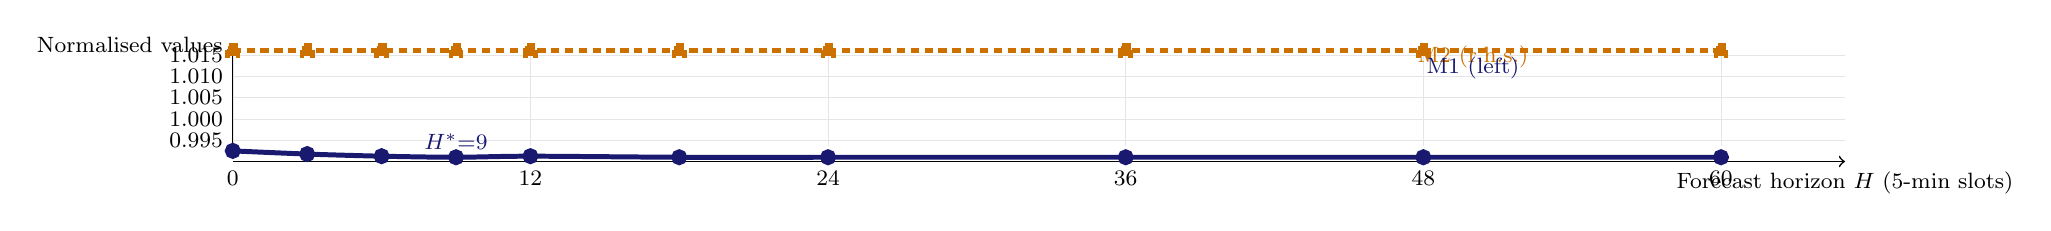
\begin{tikzpicture}[x=0.35cm, y=0.015cm, scale=0.9]
% Axes
\draw[->, line width=0.6pt] (0,0) -- (65,0) node[below, font=\footnotesize] {Forecast horizon $H$ (5-min slots)};
\draw[->, line width=0.6pt] (0,15) -- (0,110) node[left, font=\footnotesize] {Normalised values};

% Grid
\foreach \x in {0,12,24,36,48,60} \draw[black!10, line width=0.2pt] (\x,110) -- (\x,15);
\foreach \y in {20,40,60,80,100} \draw[black!10, line width=0.2pt] (0,\y) -- (65,\y);

% Tick labels
\foreach \x in {0,12,24,36,48,60} \node[below, font=\footnotesize] at (\x,0) {\x};
\foreach \y/\label in {20/0.995,40/1.000,60/1.005,80/1.010,100/1.015} \node[left, font=\footnotesize] at (0,\y) {\label};

% Data: M1 Carbon (solid line)
\draw[MidnightBlue, line width=1.8pt]
  plot[smooth, mark=*, mark size=2.2pt] coordinates {
    (0,10)(3,7)(6,5)(9,4)(12,5)(18,4)(24,4)(36,4)(48,4)(60,4)
  };
% Data: M2 SLA (dashed line) — shifted right for visibility
\draw[DarkOrange!80!black, densely dashed, line width=1.8pt]
  plot[mark=square*, mark size=2pt] coordinates {
    (0,104)(3,104)(6,104)(9,104)(12,104)(18,104)(24,104)(36,104)(48,104)(60,104)
  };

% Labels
\node[font=\footnotesize, text=MidnightBlue, anchor=south] at (9,2.3) {$H^*{=}9$};
\draw[->, line width=0.4pt, MidnightBlue] (9,3.5) -- (9,5.8);

% Legend
\node[font=\footnotesize, text=DarkOrange!80!black] at (50,98) {M2 (r.h.s.)};
\node[font=\footnotesize, text=MidnightBlue] at (50,88) {M1 (left)};
\end{tikzpicture}
\caption{Effect of the forecast horizon $H$ on carbon (M1, solid, left axis)
and SLA violation (M2, dashed, right axis). Carbon reaches a minimum near
$H=9$ slots and flattens; the SLA rate (scaled to fit the same axes) remains constant.}
\label{fig:horizon}
\end{figure}
